
% This LaTeX was auto-generated from an M-file by MATLAB.
% To make changes, update the M-file and republish this document.

\documentclass{article}
\usepackage{graphicx}
\usepackage{color}
\usepackage{listings}
\usepackage[framed]{mcode}
\usepackage{fullpage}
\usepackage{hyperref}
\usepackage{amsmath}

\definecolor{lightgray}{gray}{0.5}
\setlength{\parindent}{0pt}

\begin{document}

    
    
%\section*{}

\begin{par}

\title{BE 521 - Homework 2\\{\normalsize Spring 2015}}
\author{Mike Lautman}
\date{\today}
\maketitle
\textbf{Objective:} Computational modeling of neurons.

\end{par}
\begin{par}

\section*{1. Basic Membrane and Equilibrium Potentials (5 pts)}

\end{par}
\begin{lstlisting}
clear all; close all; clc;
warning('off');
\end{lstlisting}
\begin{par}

\subsection*{Potential Difference Vt}

\end{par}
\begin{lstlisting}
R = 8.31;       % J / (mol * K)
F = 96480;      % C / mol
Tc = 37;        % C
Tk = Tc + 273.1;% K

Vt = R*Tk/F     % 0.0267 J / C
\end{lstlisting}

\color{lightgray} \begin{lstlisting}
Vt =

    0.0267

\end{lstlisting} \color{black}
\begin{par}

\subsection*{1.2 Nernst Equilibrium Potentials}

\end{par}
\begin{lstlisting}
K_i = 400e-3; %mM
K_o = 20e-3; %mM

Na_i = 50e-3; %mM
Na_o = 440e-3; %mM

Cl_i = 52e-3; %mM
Cl_o = 460e-3; %mM


NEP_K = Vt * log(K_o/K_i)       % mV
NEP_N = Vt * log(Na_o/Na_i)     % mV
NEP_C = -Vt * log(Cl_o/Cl_i)    % mV
\end{lstlisting}

\color{lightgray} \begin{lstlisting}
NEP_K =

   -0.0800


NEP_N =

    0.0581


NEP_C =

   -0.0582

\end{lstlisting} \color{black}
\begin{par}

\subsection*{1.3a Nernst Equilibrium Potentials}

\end{par}
\begin{lstlisting}
Pk = 1.0;
Pn = 0.04;
Pc = 0.45;

Vm = Vt * log( ...
    (Pk * K_o + Pn * Na_o + Pc * Cl_i) / ...
    (Pk * K_i + Pn * Na_i + Pc * Cl_o) ...
)
\end{lstlisting}

\color{lightgray} \begin{lstlisting}
Vm =

   -0.0615

\end{lstlisting} \color{black}
\begin{par}

\subsection*{1.2.b Nernst Equilibrium at Peak Action Potential}

\end{par}
\begin{lstlisting}
Pk_peak = 1.00;
Pn_peak = 20.0;
Pc_peak = 0.45;

Vm_peak = Vt * log( ...
    (Pk_peak * K_o + Pn_peak * Na_o + Pc_peak * Cl_i) / ...
    (Pk_peak * K_i + Pn_peak * Na_i + Pc_peak * Cl_o) ...
)
\end{lstlisting}

\color{lightgray} \begin{lstlisting}
Vm_peak =

    0.0455

\end{lstlisting} \color{black}
\begin{par}

\section{2. Integrate and Fire Model (39 pts)}

\end{par}
\begin{par}

\subsection*{2.1 Modeling the membrane}

\end{par}
\begin{lstlisting}
tm = 10e-3;         % s
V0 = Vm;            % V
Rm = 10^7;          % ohms
dt = 10e-6;         % s
It = 2e-9;          % A
Vfire = -50e-3;     % V

integration_fq = 1/dt; % Hz
plot_len_s = .05;       % sec

ts = 0:dt:plot_len_s;
plot_len = length(ts);

V = zeros(1, plot_len);
V(1) = V0;
for i = 2:plot_len
    dV = (Vm - V(i-1) + Rm * It) * dt / tm ;
    V(i) = V(i-1) + dV;
    if V(i) >= Vfire
        V(i) = V0;
    end
end

figure(1)
plot(ts / integration_fq, V)
title('Integrate and Fire simulation (I=2nA)')
xlabel('Time (S)')
ylabel('Voltage (V)')
\end{lstlisting}


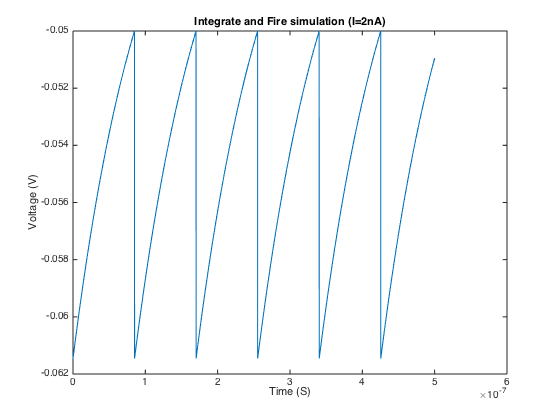
\includegraphics [width=4in]{BE521HW2_mlautman_01.png}
\begin{par}

\subsection*{2.2 Firing rate as a function of Injection Current}

\end{par}
\begin{lstlisting}
I = linspace(1e-9, 4e-9, 100);  % A
Hz = zeros(1, length(I));

time_cutoff = 20000;
for i=1:length(I)
    v = V0;
    cnt = 0;
    while v < Vfire && cnt < time_cutoff
        cnt = cnt + 1;
        dV = (Vm - v + Rm * I(i)) * dt / tm;
        v = v + dV;
    end
    if cnt >= time_cutoff
        cnt = inf;
    end
    Hz(i) = 1/(cnt*dt);
end

figure(2)
plot(I, Hz)
title('Firing Frequency vs Input Current. ')
xlabel('Input current (A)')
ylabel('Spiking Frequency (Hz)')
\end{lstlisting}


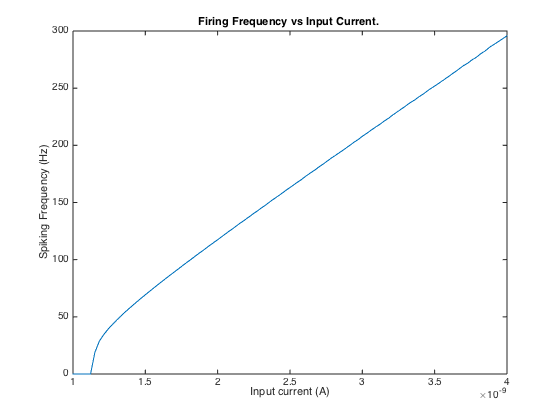
\includegraphics [width=4in]{BE521HW2_mlautman_02.png}
\begin{par}

\subsection*{2.3 Membrane voltage with dynamic Injection Current}

\end{par}
\begin{lstlisting}
dataset = 'I521_A0002_D001';
me = 'mlautman';
pass_file = 'mla_ieeglogin.bin';
[T, session] = evalc('IEEGSession(dataset, me, pass_file)');
data = session.data;
sample_f = data.sampleRate; % 200 Hz
rec_len   = data.channels(1).getNrSamples;

rec_len_s = rec_len/sample_f;           % s
I = data(1).getvalues(1:rec_len,1);     % A
dt = 1/sample_f;                        % s

V = zeros(1, rec_len);
V(1) = V0;

for i = 2:rec_len
    dV = (Vm - V(i-1) + Rm * I(i)*1e-9) * dt / tm;
    V(i) = V(i-1) + dV;
    if V(i) >= Vfire
        V(i) = V0;
    end
end

figure(3)
subplot(2,1,1)
plot((1:rec_len)*dt, V)
title('Membrane Voltage (V)')
xlabel('Time (S)')
ylabel('Voltage (V)')

subplot(2,1,2)
plot((1:rec_len)*dt, I)
title('Injected Current (nI)')
xlabel('Time (S)')
ylabel('Current (I)')
\end{lstlisting}


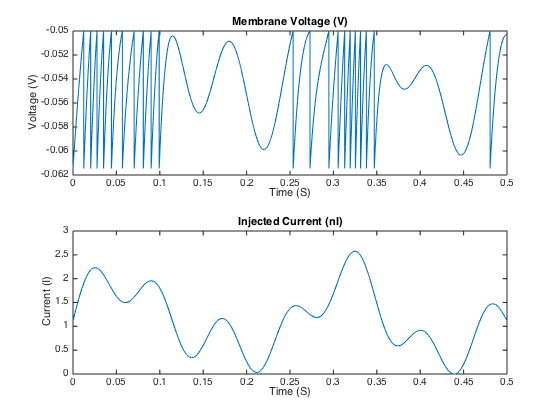
\includegraphics [width=4in]{BE521HW2_mlautman_03.png}
\begin{par}

\subsection*{2.4a Refactory Period model}

\end{par}
\begin{lstlisting}
tm = 10e-3;         % s
V0 = Vm;            % V
Rm = 10^7;          % ohms
dt = 10e-6;         % s
It = 2e-9;          % A
Vfire = -50e-3;     % V
t_sra = 100e-3;     % S
tsra = 100e-3;      % S
Vk = -70e-3;        % Volts
rm_d_gsra = 0.06;

total_t = 0.2;      % Total time (S)
t = 0:dt:total_t;

g_sra = 0;          % initial condition
rm_gsra = g_sra;

V = zeros(length(t), 1);
% V1 = V0;
V(1) = -0.0615;     % V

for i=2:length(t)

    dv = (Vm - V(i-1) - rm_gsra*(V(i-1) - Vk) + Rm * It)/tm;

    V(i) = V(i-1) + dv * dt;

    rm_gsra = rm_gsra - rm_gsra / t_sra * dt;

    if V(i) > Vfire
        V(i) = V0;
        rm_gsra = rm_gsra + rm_d_gsra;
    end
end
figure(4)
plot(t, V)
title('Integrate and Fire with Spke Rate Adaption');
xlabel('Time (S)')
ylabel('Voltage (V)')
\end{lstlisting}


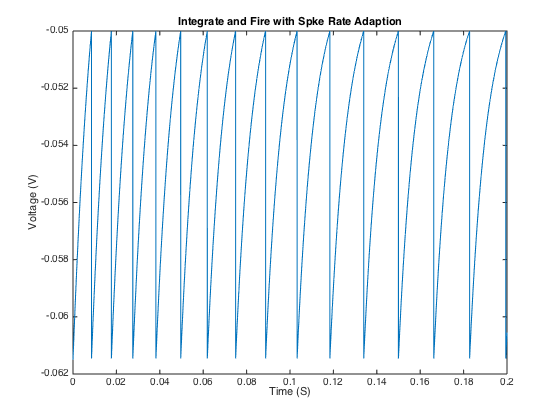
\includegraphics [width=4in]{BE521HW2_mlautman_04.png}
\begin{par}

\subsection*{2.4b Spike Interval}

\end{par}
\begin{lstlisting}
total_t = 0.5;      % Total time (S)
t = 0:dt:total_t;

g_sra = 0;          % initial condition

V = zeros(length(t), 1);
V(1) = V0;          % V

rm_gsra = zeros(length(t),1);
rm_gsra(1) = g_sra;

int = zeros(1);
cnt = 1;

for i=2:length(t)

    dv = (Vm - V(i-1) - rm_gsra(i-1)*(V(i-1) - Vk) + Rm * It)/tm;
    V(i) = V(i-1) + dv * dt;
    rm_gsra(i) = rm_gsra(i-1) - rm_gsra(i-1) / t_sra * dt;
    int(cnt) = int(cnt) + dt;

    if V(i) > Vfire
        V(i) = V0;
        rm_gsra(i) = rm_gsra(i) + rm_d_gsra;
        cnt = cnt + 1;
        int(cnt) = 0;
    end
end
figure(5)
subplot(2,1,1)
plot(t, V)
title('Membrane Voltage');
xlabel('Time (S)')
ylabel('Voltage (V)')

subplot(2,1,2)
intervals = length(int)-1;
plot(int(1:intervals))
title('Spike interval')
xlabel('Interval (cnt)')
ylabel('Time (S)')
\end{lstlisting}


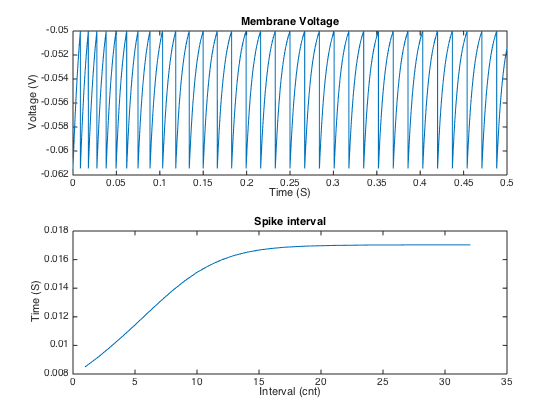
\includegraphics [width=4in]{BE521HW2_mlautman_05.png}
\begin{par}

\subsection*{2.4c Explination}

\end{par}
\begin{lstlisting}
% In 2.4b we saw that the time between spikes gradually increased athough
% those increases were decreasing. This acted like a capacitor that was
% gradually loading. The g\_sra team acts as a capacitor thus creating this
% effect.
\end{lstlisting}



\end{document}
    
